\documentclass[UTF8]{ctexart}
\usepackage{enumerate}
\usepackage{booktabs}
\usepackage{underscore}
\usepackage{graphicx, amsmath, geometry}
\usepackage[linesnumbered,boxed]{algorithm2e}
\usepackage{listings}
\usepackage{color}
\begin{document}
\title{OG阅读笔记与IBT做题技巧}
\author{寇一笑}
\date{\today}
\maketitle
\newpage
\tableofcontents
\newpage
\section{阅读}
\subsection{题型}
\begin{enumerate}[A]
\item 事实信息类问题\par
  1、再读一次,是文章细节\\
  2、矛盾的直接排除\\
  3、提及的不一定正确,必须针对题目\\
\item 否定事实类信息问题\par
  1、错误选项要么于信息矛盾,要么根本没有提及
\item 推论类问题\par
1、所选择的答案与文章主要观点不能矛盾\\
2、原文中的依据\\
\item 修辞目的类\par
1、首先知道修辞目的的单词含义,“to refute 反驳”\\
2、通常不会考整篇文章的结构,常常关注句子或段落之间的联系\\
\item 词汇类问题\par
1、不是考本身的意思,而是考在文中的意思\\
2、选出以后记得带入文中\\
\item 指代类问题\par
1、单复数和第一二三人称要一致\\
2、将所选答案替代被标示的单词或短语,检验是否违反语法规则或者是否通顺\\
3、后一个句子代词主语往往指代前一个句子的主要描述对象或者内容,通常它是主语:A does...it...\\
4、后一个分局代词主语往往指代前一个分句主要描述对象,通常它为主语:When A...,it.../a...,when it\\
5、代词的传递现象 A...it...it...\\
\item 句子简化题\par
1、两种典型错误:与被标示的句子相矛盾,遗漏了被标示的句子中的一些重要信息\\
2、不能和句子所在段落或全文主要观点相互矛盾\\

\item 句子插入题\par
1、注意逻辑关系,尤其是逻辑连接词\\
2、代词的一致性\\
\item 文章总结题\par
1、选择的一定是most important\\
2、错误的选项包括:细节、less important、与文章内容矛盾\\
\item 表格填写题\par
1、抓主要/核心观点,次要的观点一般都是为了支持主要的观点的\\
2、通常不只有一个核心观点,这类文章有几种典型结构:对照-对比、问题-解决方法、原因-结果、论点-切换(如理论、假设)等等\\
3、错误的答案可能包含了文中没有提到的话题、或者与表格中的类别不直接相关的信息;同样可能市基于文中提到的信息走出的明显错误的推断或总结\\
\textbf{注意:错误的选项同样可能会含有写文章中的原词或原句}
\end{enumerate}
\subsection{做题技巧}
\begin{enumerate}[A]
  \item 词汇题\\
  利用词根词缀猜测词性\\
  \item 句子指代题\\
  \begin{itemize}
  \item 意群划分法\\
\textbf{画意群第一个出现的名词性单词,短语或句子的主语,连词、介词、标点前停顿,and,but左右结构一致。错误选项有:}\\
  1、 细节当作主干讲\\
  2、 没有的信息,错误的信息\\
  3、 增加绝对词语\\
  4、 简单句请找主干\\
  \item 找准逻辑\\
  因:in that,due to, owing to\\
  果:so that,hence,accordingly,contribute to,be attributed to,result from\\
  转折:instead,while\\
  递进:beyond that\\
  vice versa 反之亦然\\
  \item 并列要找全\\
  \item 主从分开核对\\
  \item 正确选项包括主干内容,是同义替换,有主干逻辑,错误选项:错误,无中生有、遗漏\\
  \item 没必要读全文\\
  \end{itemize}
  \item 事实信息类问题\\
  \begin{itemize}
    \item Steps\\
    1、读题干:关键词(相关内容)+考点词(问什么)\\
    2、读原文:关键词(定位点)+考点词(答案),考点据不一定跟定位句为同一句\\
    3、正确选项是同意替换,不要推理\\
    4、排除错误选项:曲解文义,无中生有(比较级,最高级,绝对词),答非所问\\
  \end{itemize}
  \item 反事实信息题\\
  句内几种列举、段内集中列举、段内分散列举,关键在于排除。
  \item 事实推断题\\
  \begin{itemize}
    \item Steps\\
    1、读题干~关键词\\
    2、读原文~定位\\
    3、读选项~直选\\
  \end{itemize}
  \item 目的题\\
  \begin{itemize}
   \item Steps\\
    1、读题干,找到定位句\\
    2、读原文,都上下文,找到服务句,分析关系\\
    3、正确:与服务句子关系+同义替换\\
  \end{itemize}
  \item 句子插入题\\
  \begin{itemize}
  \item Steps\\
    1、先读插入句,进行预判\\
    2、读原文,寻找预判\\
    3、不要看一个,放一个,看完ABCD再寻找预判\\
    4、代入验证,前后相接\\
    \item 预判方法\\
    代词,连接词,重复,逻辑关系\\
    \item A选项一般不选,一般开头是主旨句,代词前的空一般不选\\
  \end{itemize}
  \item 修辞目的题\\
  \begin{itemize}
    \item 段内结构\\
    画连接词,分析句子间关系
    \item 段落目的\\
    总分,转折,递进
    \item 段落间关系\\
    解释、递进、转折
    \item 修辞目的题\\
1、不需要通读全文\\
2、找到例子$\rightarrow$找到观点$\rightarrow$找同义替换\\
  \end{itemize}
  \item 6选3\\
  \begin{itemize}
    \item 正确——main ideas,错误——not mentioned+details
    \item 明显错误/未提及——排除两个,似对非对——验证两个,main idea——直选两个
    \item main idea 标题、首段、主体段开头,注意文章常常没有结尾
    \item 做题时可以尝试每段总结一个关键词
  \end{itemize}
\end{enumerate}
\subsection{其他注意事项}
\begin{enumerate}[A]
  \item 题干——段落定位精读,时间紧张
  \item 略读——理解大意(有重点读),抓住主干、逻辑关系词、首段每段开头两句
\end{enumerate}
\subsection{经验总结}
\begin{enumerate}[A]
  \item 不出题的段落也会考,在最后几题出现
  \item 没必要逐句翻译,时间会不够的,可以先读题干,再带着目的or方法阅读文章
  \item 13题20分钟,最后两题五分钟
  \item 最后一题区分main idea和detail
  \item 第一题进入状态要快
  \item 有时间背一下阅读的单词题
  \item 句子插入题注意指示代词 that/this
  \item 细节题注意题干问什么
  \item 最后一题,第一段可能因为提及太小被当做细节,两个观点可能因为提及过多而不能简短总结
  \item 最后一题,分类,依据要从原文找
  \item 最后一题,每段看完记录一个原文的词语
  \item 句子简化题,找清楚两个句子成分的关系(比如谁是主要,谁是次要)
  \item 碰到复杂的学术名词,注意看小括号的解释
  \item 事实信息题:先看选项的关键词(一些无法被同义替换的专业词语),再到文章中找定位,解题会快
  \item 否定事实信息题:从选项中找到关键词,回到原文中定位用排除法
  \item 功能目的题,上下文定位
  \item 句子简化题,注意逻辑关系
  \item 最后一题,比起判断是否是细节,更优先判断是否错误/没有提到的信息
  \item 词汇题,直选+排除
  \item 区分事实信息题和推断题,事实信息题不要过分推断
  \item 最后一题最好是排除选出的
  \item 修辞目的题,为什么要写这段话,要分清大的目的和小的(一般满足大的),注意选项可能会对小的做一个混淆
  \item 主旨题可能会出现在中间内容,承上启下
  \item 特别留意说明来意的句子
  \item 留意完全陌生的学术名词,可能出why mention题目
  \item 功能目的题的举例,一般和前文内容有关
  \end{enumerate}
\section{听力}
\subsection{lecture的话题类别}
\begin{itemize}
  \item 艺术
  \item 生命科学
  \item 自然科学
  \item 社会科学
\end{itemize}
\subsection{题型}
\begin{enumerate}[A]
\item 内容主旨题\\
1、内容主旨题考察的市讲座或者对话的总体内容,排除那些只涉及局部听力材料的选项\\
2、试用一个短语或一句话概括讲座或对话的主题\\
\item 目的主旨题\\
1、学生去找教授可能有各种各样的目的,应根据笔记找出最初目的\\
2、对话的目的不总是跟着对话的主要内容相关。有可能突然引出来的话题\\
3、学生服务问题抓住主要的问题所在\\
\item 细节题\\
1、回答问题时参看笔记。题目不会考察考生一些小的细节。笔记内同应该包括对话或者讲座中的重要细节\\
2、错误选项中有可能包含听力材料中有的词组\\
3、如果无法确定正确选项,就选择一个与讲座或对话的主题最符合的选项\\
\item 句子功能题\\
说话人的字面意思可能与真实意图不符
\item 说话人态度题\\
抓住说话人的语气,注意反语
\item 组织结构题\\
包括整个讲座的组织方式、两个不同观点之间的关系、某一句话的功能\\
\item 连接内容题\\
填表题/排序题
\item 推论题\\
正确答案往往用到了讲座或者对话中未提到的词汇\\
\end{enumerate}
\subsection{如何训练听力}
\begin{enumerate}
  \item 将mainidea,major points,important details在纸上分行列出,提醒自己在听听力材料的时候要注意这几个方面并记笔记,反复听录音材料,直到写下所有重要的观点和细节
  \item 先听讲座的一部分,听完以后写出译者主要观点的简短总结;再逐渐增加所听部分的长度进行总结
  \item 思考讲座稿的谋篇布局。注意听清听清听力材料的标志词,他们会标明文中的引言、主要步骤和观点、例子、结论及总结
  \item 注意听那些能表示观点之间联系的词汇,弄清材料中观点之间的联系,可能涉及因果,对比,过程中的步骤等
  \item 听完录音以后,写出一个所听到内容的提纲
  \item 注意听出说话人的话题转换,说话人再简短讲了一些题外之话之后再次回到正题上
\end{enumerate}
\subsection{听力技巧}
\begin{itemize}
\item 纵向记笔记\\
\item 顺序出题\\
\end{itemize}
\subsection{新托福听力金牌教程}
\subsubsection{题型}
\begin{enumerate}[A]
  \item Main idea\\
  \begin{itemize}
    \item 关键词会在开头出现(信号词、句)
    \item 关键词不一定是具体答案(注意细节描述)
    \item 选项中可能都会涉及关键词
    \item 两类典型错误:内容不符和以偏概全
  \end{itemize}
  \item Detail\\
  \begin{itemize}
    \item 细节题一定会围绕文章的中心问题
    \item 记录举例的特征、例子及原理
    \item 正确答案经过paraphrasing
    \item 典型错误
    \begin{itemize}
      \item not correct
      \item not mentioned
      \item not related to question
    \end{itemize}
  \end{itemize}
  \item Function
  \begin{itemize}
    \item 题型
    \begin{itemize}
      \item 理解说话者的意图
      \item 理解表达的含义
    \end{itemize}
    \item 理解情景非常重要 p60
    \item 熟悉表达说话者意图的各种动词
  \end{itemize}
  \item Attitude
  \begin{itemize}
    \item 语气词
    \item 动词的情感
    \item 典型错误(表层含义和深层含义)
  \end{itemize}
  \item Organization\\
  \begin{itemize}
    \item 提前预测哪些要点会成为问题
    \begin{itemize}
      \item 讲义文的开头和结尾部分
      \item 说明新概念的部分
      \item 看起来与正文关联部分不大的例子或比喻出现的部分
    \end{itemize}
    \item 讲义文的中基本叙述方式(整体、局部)
  \end{itemize}
  \item Connecting contents\\
  \begin{itemize}
    \item 题型
    \begin{itemize}
      \item 特征——yes or no
      \item 项目——分类
      \item 事情发生顺序
    \end{itemize}
  \end{itemize}
  \item Inference
  \begin{itemize}
    \item 推导,但要在文章中找到依据
    \item 对原文的重复不算是正确答案
  \end{itemize}
\end{enumerate}
\subsection{知乎live}
\begin{enumerate}
  \item Conversation有结构
  \begin{itemize}
    \item 打招呼
    \item 说明来意 -- Q1 why come?
    \item 分析问题 -- Q2
    \item 解决方案(担忧) -- Q3
    \item 最终解决方案 -- Q4 What next
  \end{itemize}
  \item Lecture有结构
  \begin{itemize}
    \item 引入部分\\
    1、开门见山\\
    2、回顾一下上一节课的内容\\
    3、闲扯半天\\
    \textbf{然后会有一段对于学科词汇的解释,这个很重要}
    \item 展开讨论\\
    第一种(理科)\\
    1、总起(比如:有很多theory)\\
    2、分述(各种观点)
    第二种(文科)\\
    直线型\\
  \end{itemize}
  \item 结构有用
  \begin{itemize}
    \item 引入话题
    \item 话题+定义/解释
    \item 总起
    \item 分点1 Q2
    \item 分点2 Q2
    \item 分点3 Q3
    \item 总结     Q5
  \end{itemize}
  \item 做题方法
  \begin{itemize}
    \item 跨区排除\\
    顺序出题,题干在哪个区,选项一定在哪个区
    \item 左上右下\\
    why mention? 右下的例子是为了阐释左上的内容
  \end{itemize}
\end{enumerate}
\subsection{经验总结}
\begin{enumerate}
  \item 注意细节题会列举哪些东西
  \item 听力之间没有间隔
  \item 学术词汇要牢记,tpo5的spectrum
  \item 举例阐述的时候会考作用题,虽然这个例子(zinc)可能不认识(e.g.这个例子和哪个例子对比)
  \item 两者相互对比记录特征的时候,要注意主语,在后一部分可能经常提到前者
  \item 听力的选项是同义替换(compliment-feedback),不一定没有听到
  \item 列举一大堆名词的时候会考细节题
  \item last week, we cover(提到了) some arguments
  \item ok,shoot(说吧)
  \item 细节题可能会考他的research topic
  \item 听力选项看全,逐个排除
  \item 除了听清要做什么事情,还要听清里面的细节(工具)
  \item 最后一句话也要好好听,非常有可能出题目
  \item conversation 信号词: that's kind of what want to talk to you about
  \item 笔记可以潦草一点
\end{enumerate}
\section{写作}
\subsection{综合写作}
\subsubsection{阅读文章和讲座的关系}
\begin{enumerate}
  \item 总结概括讲座中的要点,解释这些要点如何对阅读文章中的某些具体观点产生怀疑
  \item 总结概括讲座中的要点,解释这些要点如何对阅读文章中的某些具体观点提出质疑
  \item 总结概括讲座中的要点,解释这些要点如何对阅读文章中提出的问题做出回答
  \item 总结概括讲座中的要点,准确说明这些要点如何支持阅读中的解释性论述
  \item 总结概括讲座中的要点,准确说明这些要点如何加强阅读文章中的某些具体观点
\end{enumerate}
\subsection{怎样做题}
\textbf{在阅读文章时:}
\begin{itemize}
  \item 再草稿纸上作笔记
  \item 找出文章的中心思想,中心思想通常是与某一问题的政策、实践活动、或者与某一问题的立场有关,也可能是对某些行为过程或者某些自然现象的产生作出的一些概括性假设。
  \item 了解作者是如何评价并展展开中心思想的。展开中心思想通常有以下俩种方式:
  \begin{enumerate}
    \item 用议论性或说明性语言支持中心思想。例如:说明为什么有理由相信某些政策或时间行为是有益的;或正式这些政策、时间行为是有用的、明智的;或者说明为什么某些政策或事件行为再过去是好的。
    \item 用议论、说明或者提出问题的方式引出人们关心的问题———为什么某种政策、时间行为立场行不通、不明智
  \end{enumerate}
  \item 不要记住阅读文章中的内容。在开始写作时,阅读文章会在屏幕上再次出现。
  \item 既要注意文章张那些支持中心思想的论点,也要注意那些对中心思想提出质疑的论点。通常,中心论点会通过三点展开。
\end{itemize}
\textbf{在听听力短文时:}
\begin{itemize}
  \item 在草稿纸上作笔记
  \item 努力听出那些使阅读文章中的观点看起来粗无、不具有说服力甚至不真实的信息、事例或者解释。
\end{itemize}
\textbf{在写作过程中}
\begin{itemize}
  \item 开始写作时再读一遍短文,参考笔记,列一个写作提纲。可以将提放列在草稿上,也可以再阅读文章和讲座的笔记上画出重点,还可直接将提纲和笔记键入屏幕上
  \item 综合写作不要求考生发表个人观点,而是让考生解释说明讲座中的观点是如何与阅读文章张观点联系在一起的
  \item 写出完整的英语句子。作文中要列出阅读文章与讲座张相独立的观点。可以写成一个长段落,也可以写成几个短段落。偶尔出现语言错误,只要不对表述的观点产生误解,就不会影响作文成绩。
  \item 牢记自己的任务是从讲座中跳出与阅读文章相关的重要信息,并将这些信息连贯,准确的在作文中表述出来。作文应符合下列要求:
  \begin{enumerate}
    \item 包含讲座中的一些确切观点、解释说明和议论。这些内容恰好对阅读文章中的观点提出质疑或与其相反。
    \item 陈述各观点时要连贯、准确。
    \item 条理清晰,结构连贯。这样的作文能够使读者理解将讲座中的观点与阅读文章中的观点使如何相互联系的。
    \item 作文长度使150-225词.只要作文回大理实体的问题,字数多也不会扣分。
  \end{enumerate}
  \textbf{如果作文全部使找阅读短文抄下来的,得零分;如果只写了有关阅读文章的观点,得1分;要写出高分作文,必须写清楚讲座的观点使如何与阅读文章的一些具体观点相联系的。}
\end{itemize}
\subsection{独立写作}
\subsubsection{Tips}
\begin{itemize}
  \item 动笔前要思考。在草稿纸上列提纲或者记笔记,以帮助组织思路。也可以直接将提纲和笔记键入屏幕中答案区域,然后即将这些内容写成句子或者段落,写尽自己的论文
  \item 掌握时间。尽可能在倒计时还剩4-5分钟结束写作,用剩余时间检查所写内容,并作最后的修改。
  \item 写作时,不要死记硬背下来的例子或者论证。
\end{itemize}
\subsubsection{打分标准}
\begin{enumerate}[A]
  \item 展开观点\\
  用各种支持内容(包括事例、细节、理由等)来支持文章的观点。要得高分,就要按照评分指导的原则写作文——“很好的展开论点、运用恰当清晰的解释、例证和斜街”。评分人会根据考生的作文是否切题,文章中的细节、事例、理由在多大程度上支持了论点。注意,不要仅仅为了增加文章字数而背一些冗长的段落,堆砌大量词语却没有针对论点展开论述的话。一定要对所给话题的一些具体观点展开论述。
  \item 文章结构\\
  分段写作并在两个观点只见那运用过渡可以帮助读者跟上作者的思路,但要直到,仅仅使用“first”、“second”这样的连接词并不能保证作文结构的严谨,还要注意让所有的观点与文章的主题相关,紧扣中心思想。评分标注提到的统一性、渐进性、连续性——就是要结构严谨。要获得高分,需要避免累赘、离题以及条理不清晰的衔接。
  \item 语言运用\\
  要获得高分,作文要体现“语言运用的和谐流畅”,作文的句子要结构多样,措辞要贴切得体。
\end{enumerate}
\begin{enumerate}[A]
  \item 独立写作
  \begin{itemize}
    \item 思路展开(利弊/原因/分类说明)
    \item 审题注意限制对象,e.g. children
    \item 结构:一个观点+两个分论点
    \item 9个常用角度
    \item 例子:如何让教师的课堂更加有趣
    \begin{itemize}
      \item 技术:优点是知识形象生动 缺点:分散注意力
      \item 讨论: 1、人们更容易讨论发表自己的意见,更加自由 2、可以有氛围,带动懈怠同学 缺点1、gossip 2、被懈怠同学影响
      \item 新闻 优点1、现实
    \end{itemize}
    \item 开头段(60-80)
    \begin{itemize}
      \item 开头不要太简单,直接写出自己的观点
      \item 必须有观点
      \item 引入 + 正反(复述题目)+ 观点讨论 + 我认为(提出主论点),其中引入避免with the development of
      \begin{itemize}
        \item 复述题目 疑问句
        \item 对比的时候只写反方观点
      \begin{figure}[!htp]
        \centering
        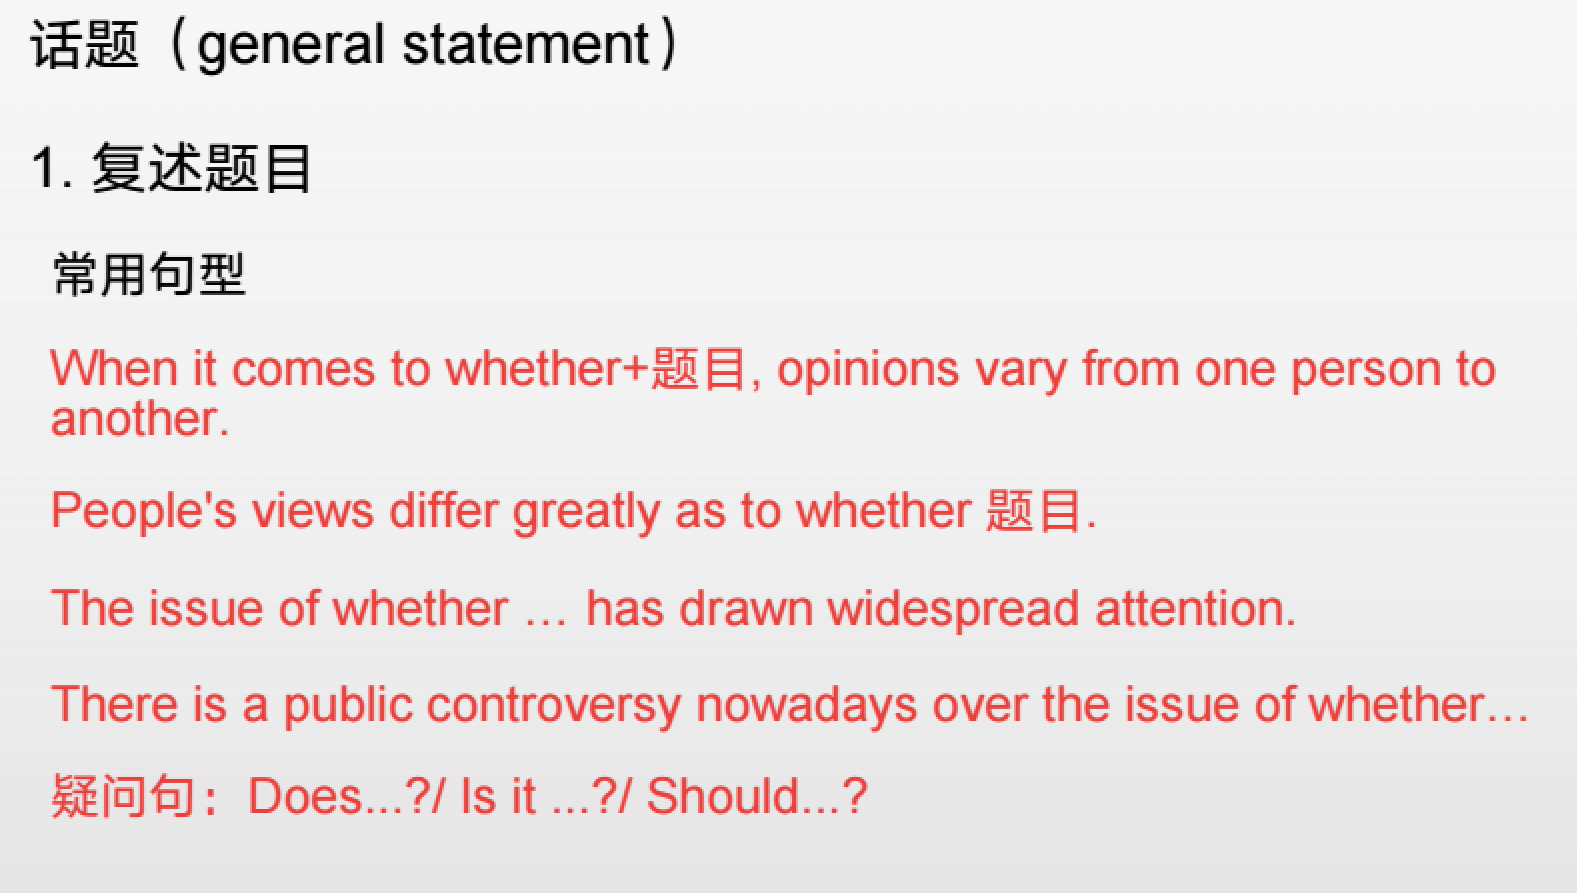
\includegraphics[width=4.00in,height=3.00in]{xiezuo1.png}
        \caption{引入常用句式}
      \end{figure}
      \item 反方观点
            \begin{figure}[!htp]
        \centering
        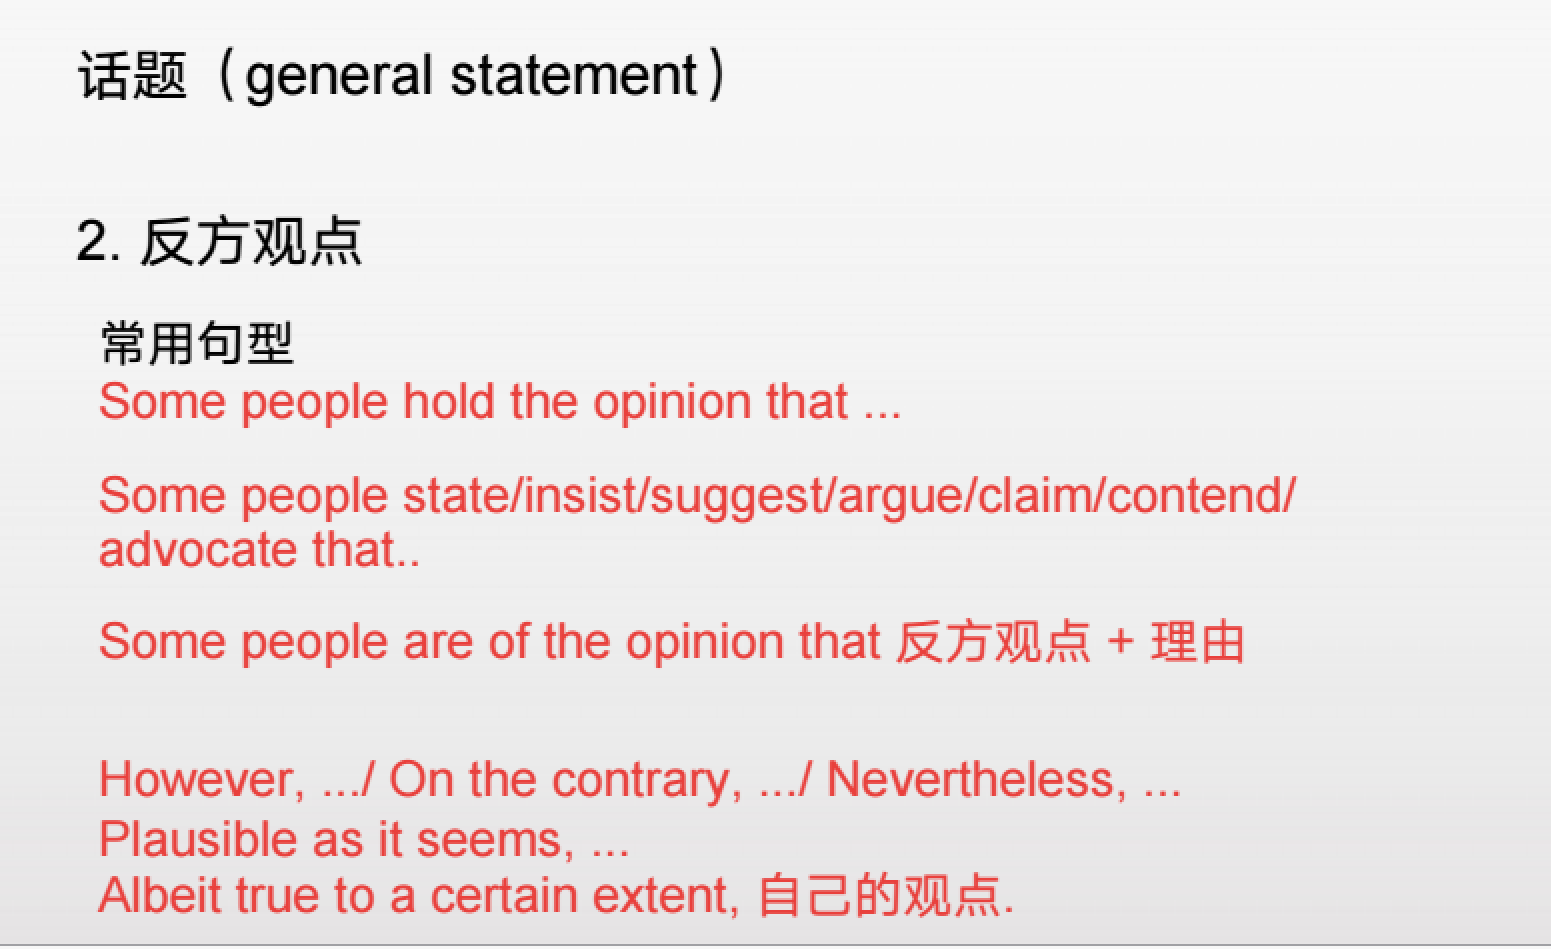
\includegraphics[width=4.00in,height=3.00in]{xiezuo2.png}
        \caption{反方观点句式}
      \end{figure}
      \item 自己的观点
                  \begin{figure}[!htp]
        \centering
        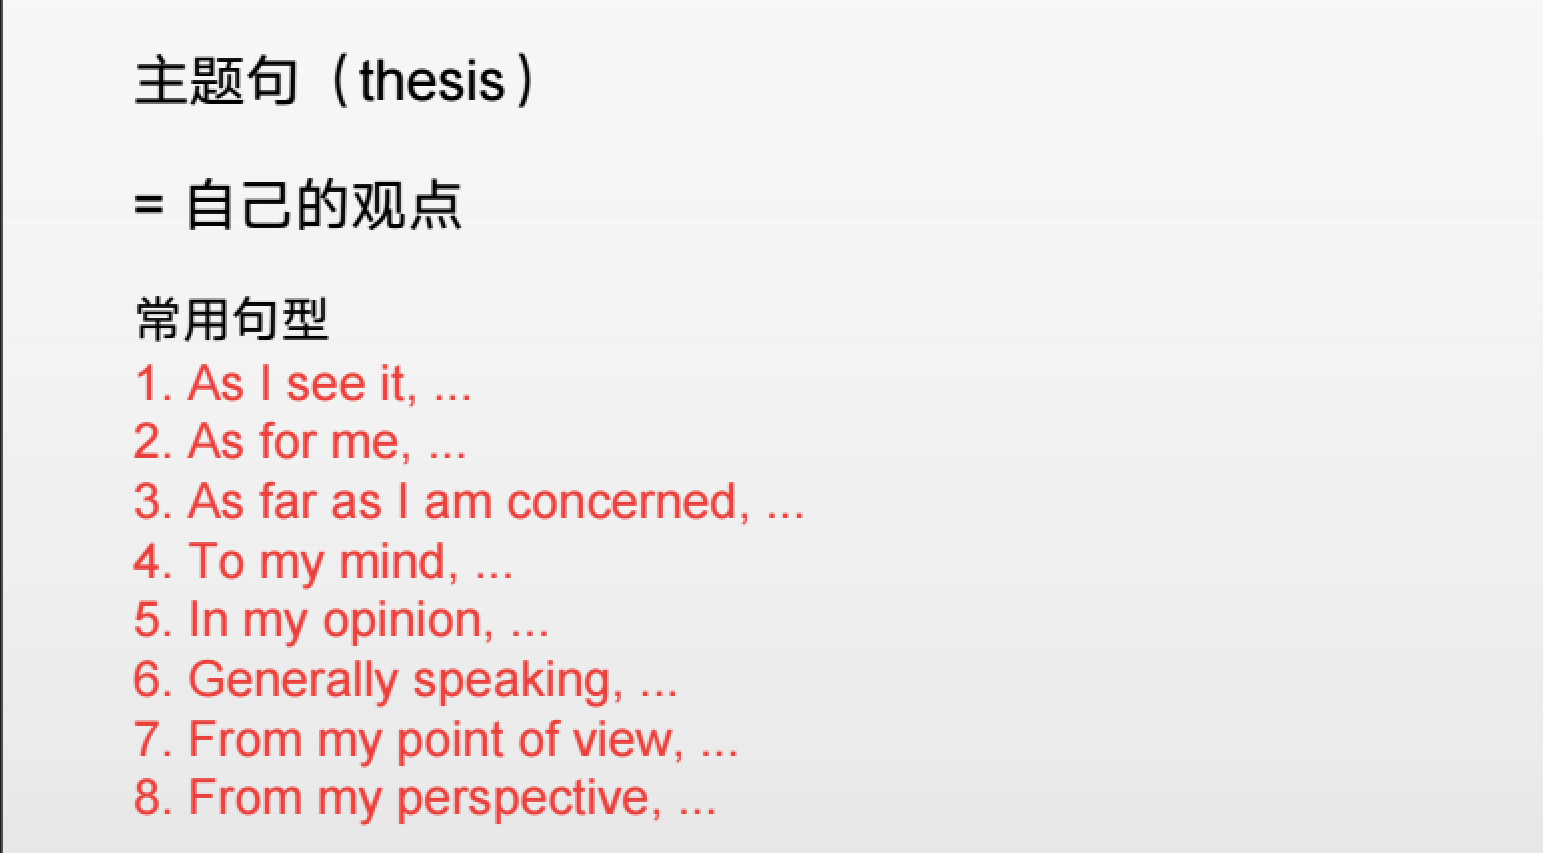
\includegraphics[width=4.00in,height=3.00in]{xiezuo3.png}
        \caption{反方观点句式}
              \end{figure}
      \end{itemize}
      \item 同义替换
                        \begin{figure}[!htp]
        \centering
        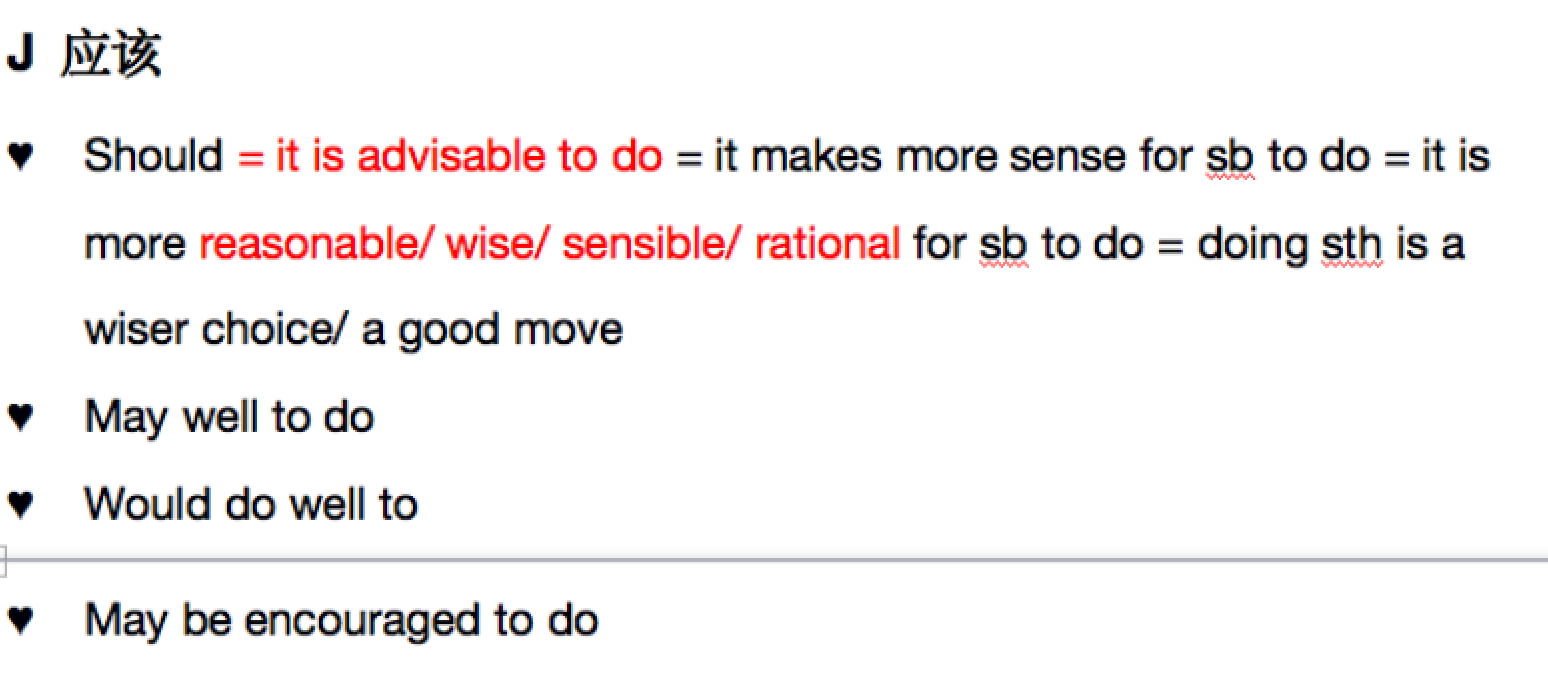
\includegraphics[width=4.00in,height=3.00in]{xiezuo4.png}
        \caption{should同义替换}
              \end{figure}
      \item 3-5分钟,50-100词,要点全面,展现语言功底
      \item 人称不要用第二人称,可以用第一或者第三人称,显示正式化
      \item 引入:话题词/问题 + 展开(原因/好处/并列细节) \\
      话题词 定义/重要/普遍/备受关注/重大影响
                              \begin{figure}[!htp]
        \centering
        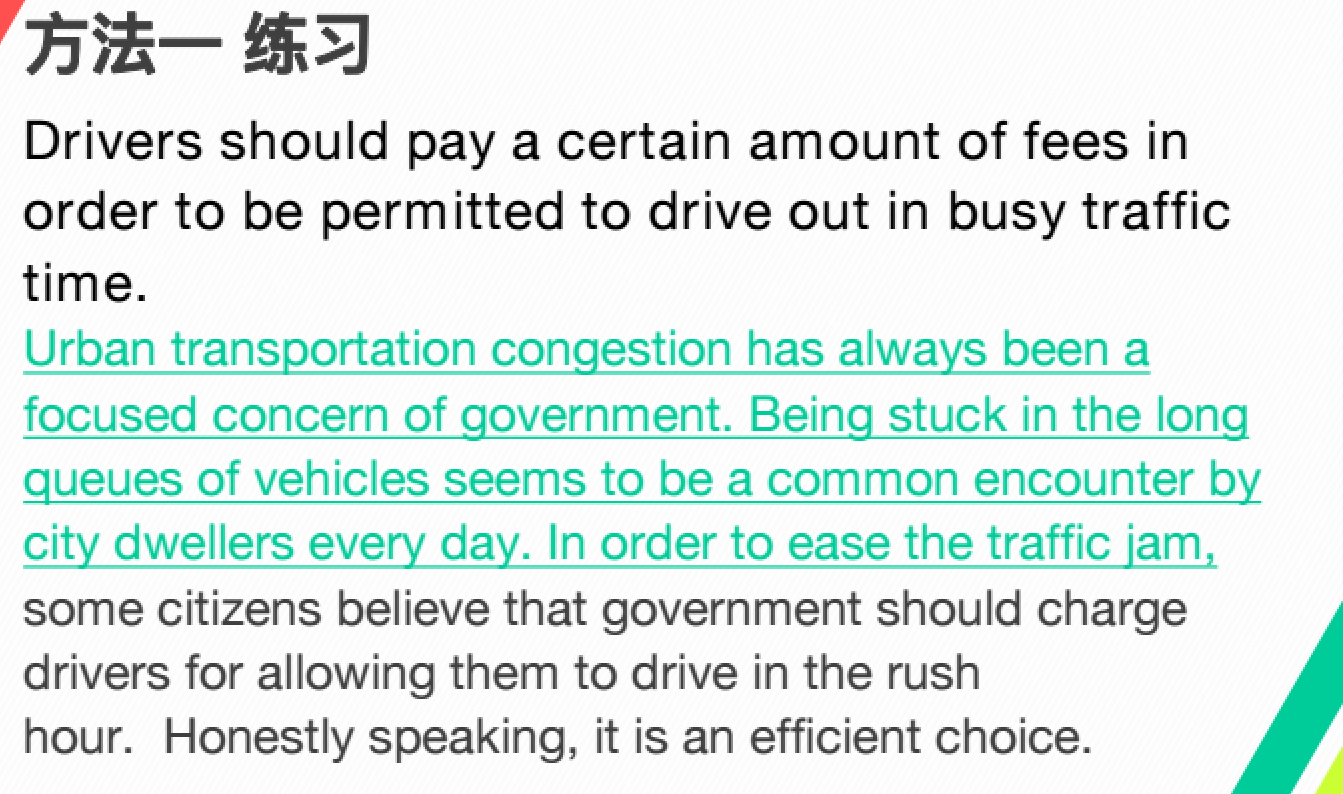
\includegraphics[width=4.00in,height=3.00in]{xiezuo5.png}
        \caption{以问题入手}
              \end{figure}
        \begin{figure}[!htp]
        \centering
        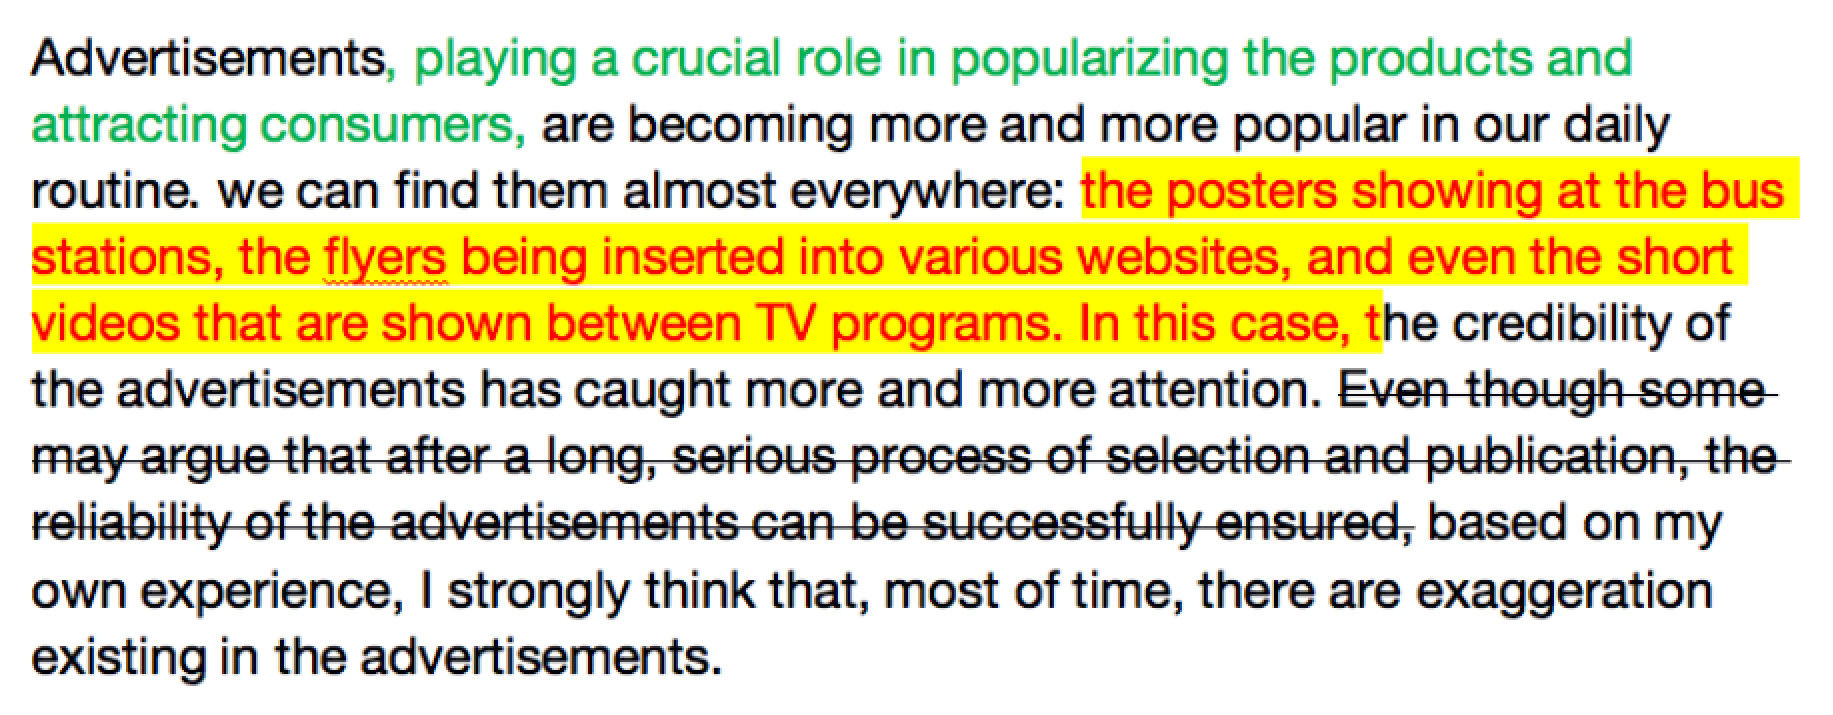
\includegraphics[width=4.00in,height=3.00in]{xiezuo6.png}
        \caption{以话题入手}
              \end{figure}
    \end{itemize}
    \item 开头段不要太多比较优劣,占用主体段的内容
    \item 反方观点可以不写,不要用自己的观点去引用,推荐用交叉的一点或者写反方然后去反驳
    \item 区分背景句子和话题句子
    \item 二选一,(whether ... or ... is beneficial)
            \begin{figure}[!htp]
        \centering
        
\includegraphics[width=4.00in,height=3.00in]{xiezuo7.png}
        \caption{例子}
              \end{figure}
  \end{itemize}
    \item 主体段(120-150)
    \begin{itemize}
      \item 结构: 主题句+解释论证+举例论证+总结
      \item 主题句
            \begin{itemize}
        \item 言简意赅
        \item 拒绝假大空,要实际
        \item 没有必须多少字的要求,要把细化的东西、逻辑写好
        \item 对比问题,万能理由不成立
        \item xx导致xx,方向要大,一句话,论证中心,可拆分成两个方面
        \item 好处要与主题有相关性,多个老师应从教育出发,而不是锻炼沟通能力
        \item 拆分:人类活动破坏地球 哪些人类活动 地球:空气 水
        \item 写缺点,最好是两个优点主体,一个缺点作为附属,只写一个优点一个缺点会很贫乏
        \item 不要摆事实,要摆影响,细节后面写
        \item 主题句可以培养品质,然后后面可以细化并列
        \item 从不同角度来讲,学生家长学校,工作生活学业
        \item 直接说出主旨
        \item 减少铺垫
        \item 要把一些生活的原理说明白,不要理所当然
        \item 论证的逻辑、主题和主题句子要一样
        \item 回扣句要和主题一样
        \item 尽量不要对比,对比的铺垫和细节无关
        \item 横向多拆解一下,多方面体现,让主题能够充分体现
        \item 但也不要光而不精,只有例子没有细节不可以
        \item 次序句+主题句+(解释句)+论证法展开的论证细节+回扣句\\
        解释句:\\
        1、背景铺垫 2-3 主题句 带一个引出背景的议论文句式\\
        2、让步 对方在主题句限制的范围下的好处,不要说自己的缺点\\
        3、解释细化主题句,涉及论证中心的转移(细化) in other words / to be more specific\\
        \item 论证方法\\
        个人事例、对比、逻辑说理、细节、让步驳论\\
        \item 利弊类主题句:观点(关键词)will/can 好处+坏处\\
        xxx is a good way to ...\\
        xxx will exert a negative impact on\\
        观点不要用it来指代 \\
                    \begin{figure}[!htp]
        \centering
        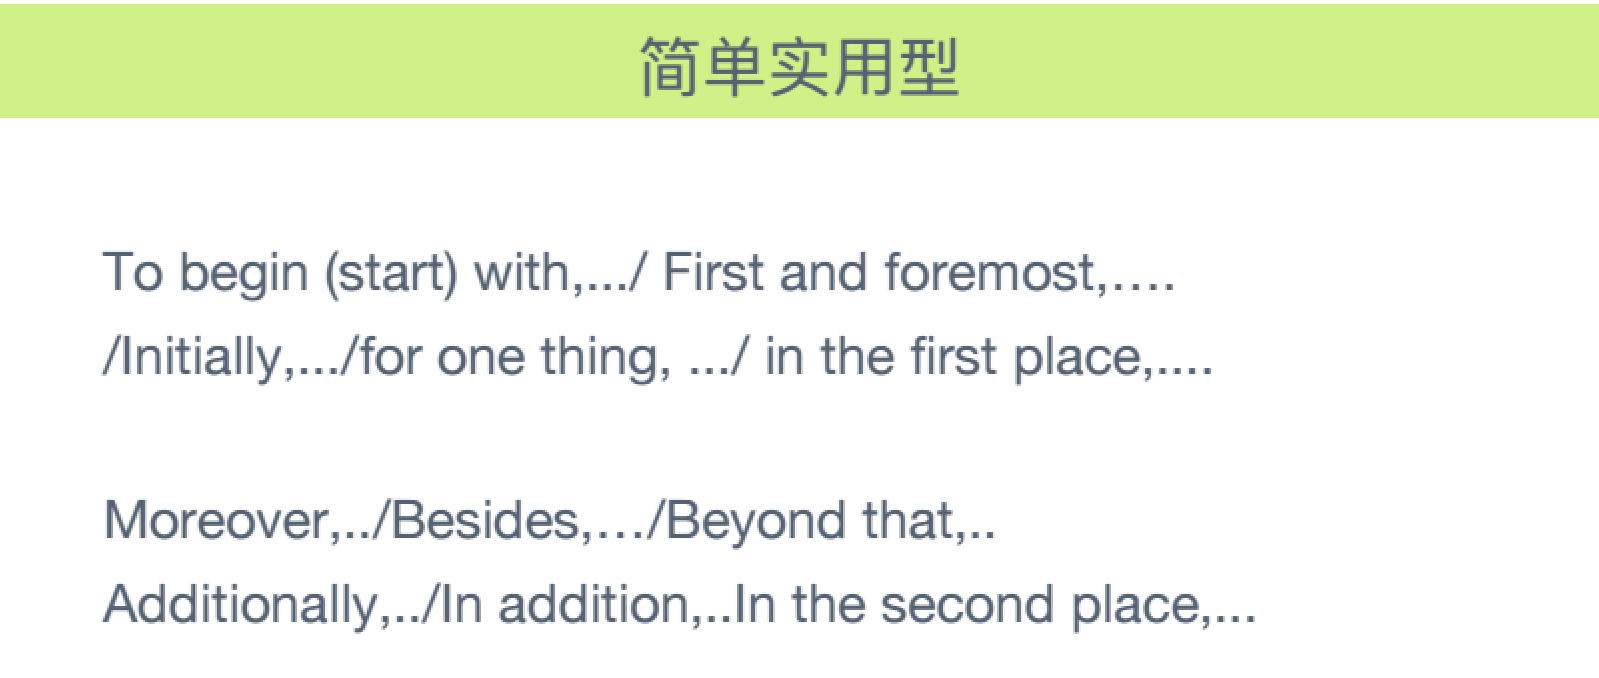
\includegraphics[width=4.00in,height=3.00in]{xiezuo8.png}
        \caption{序列词1}
              \end{figure}
              \begin{figure}[!htp]
        \centering
        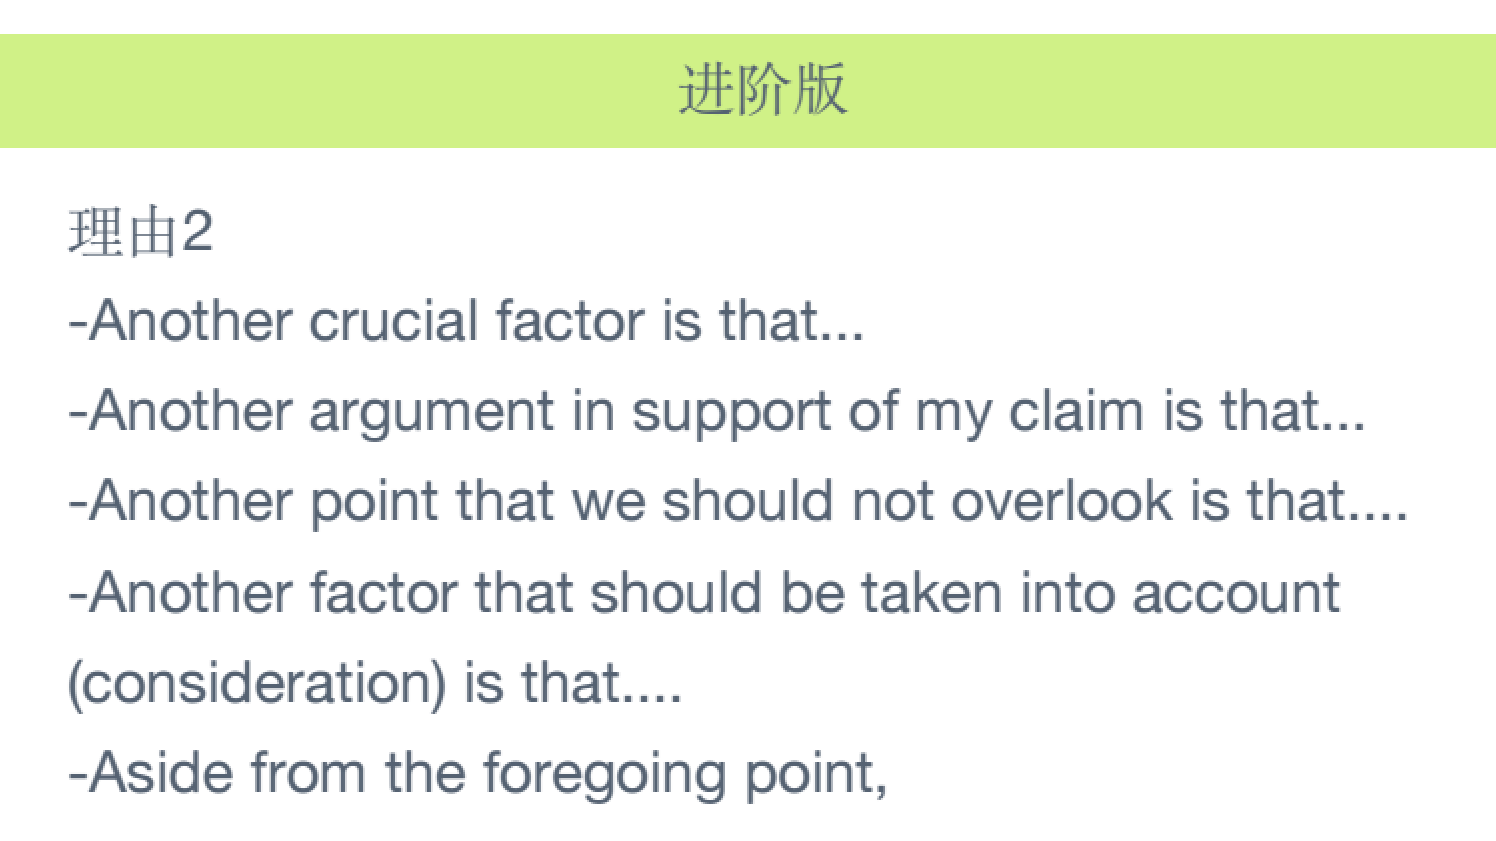
\includegraphics[width=4.00in,height=3.00in]{xiezuo9.png}
        \caption{序列词2}
              \end{figure}
        \item 解释主题句--观点 带来 好处-- 结论\\
        原因 导致 观点 对于细节可以展开 \\
        因:为什么需要这个--问题/现状/重要(optional,看题目)\\
        果:重中之重:解释起点是如何如何如何到终点,注重逻辑完整(necessary)\\
        \begin{figure}[!htp]
        \centering
        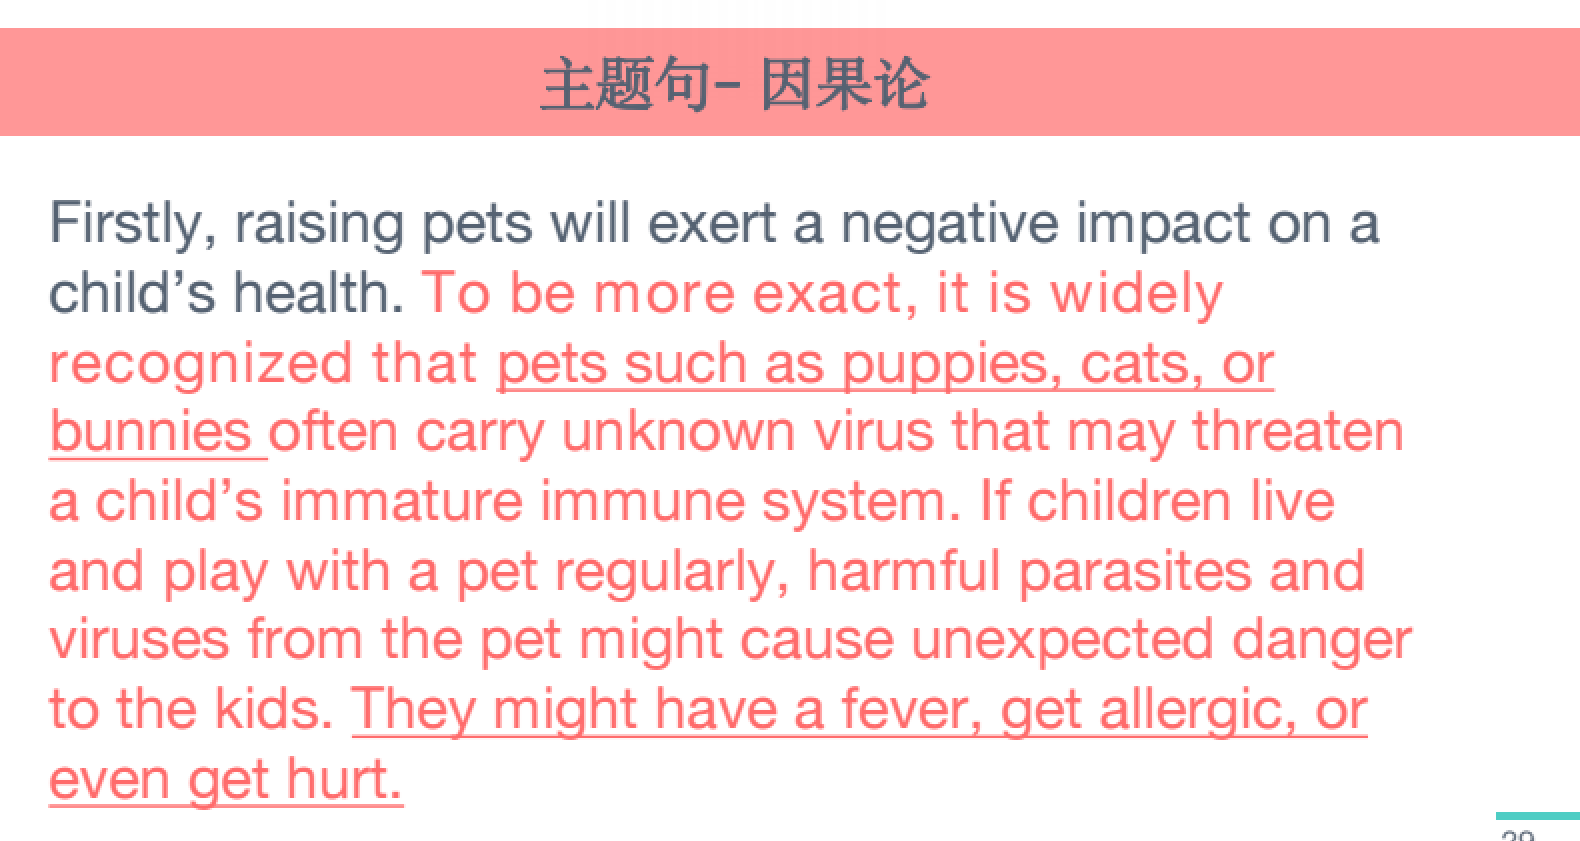
\includegraphics[width=4.00in,height=3.00in]{xiezuo10.png}
        \caption{原因-->结果}
              \end{figure}
              \begin{figure}[!htp]
        \centering
        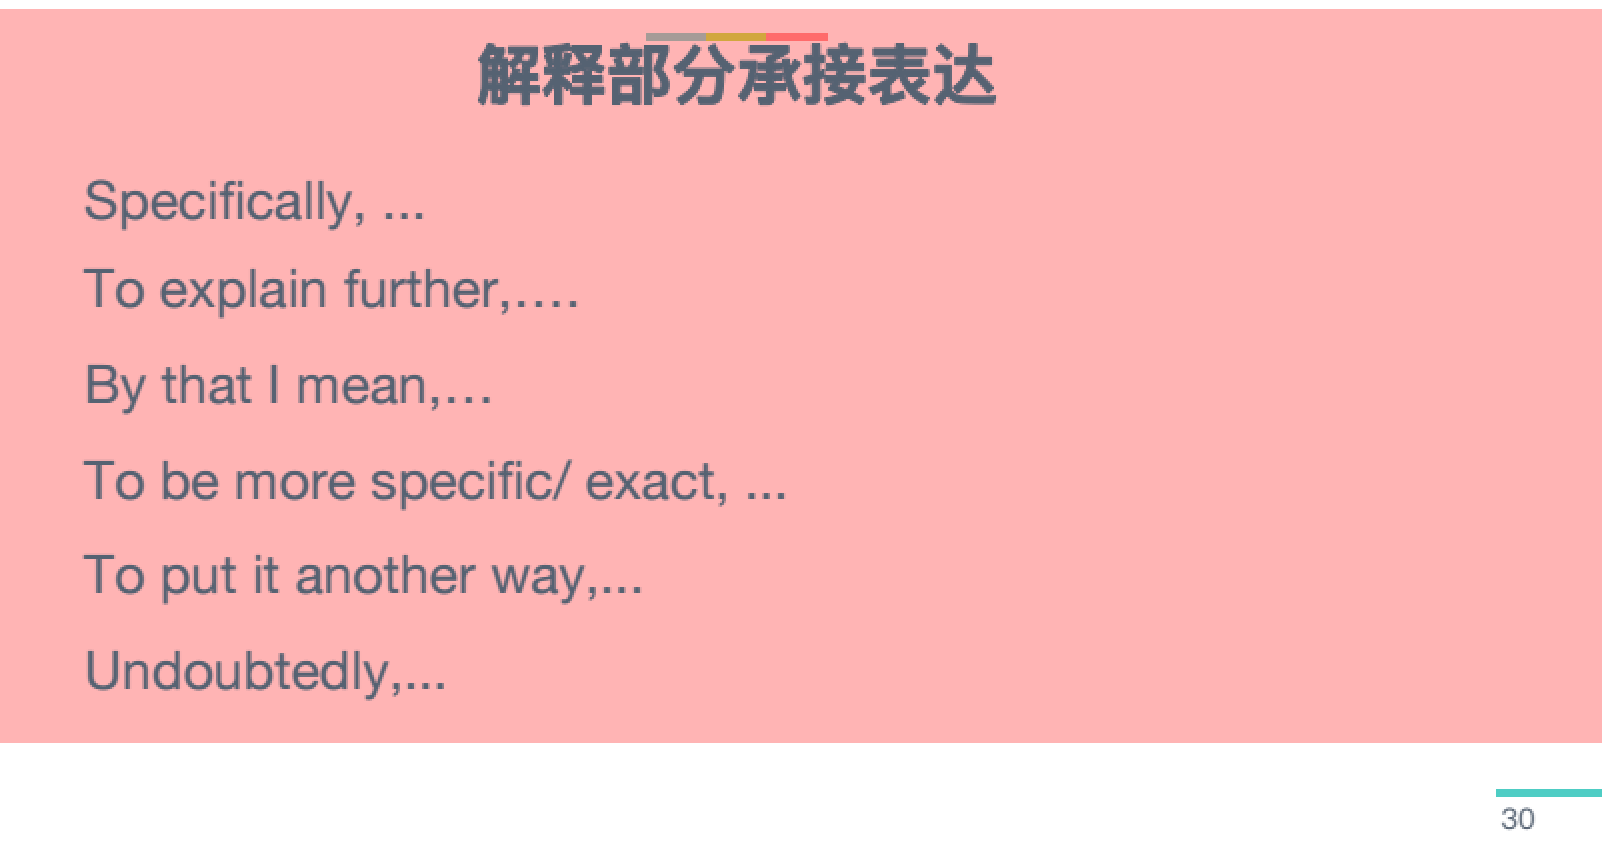
\includegraphics[width=4.00in,height=3.00in]{xiezuo11.png}
        \caption{解释部分承接词}
              \end{figure}
      \end{itemize}
      \item 标点符号空一格
                    \begin{figure}[!htp]
        \centering
        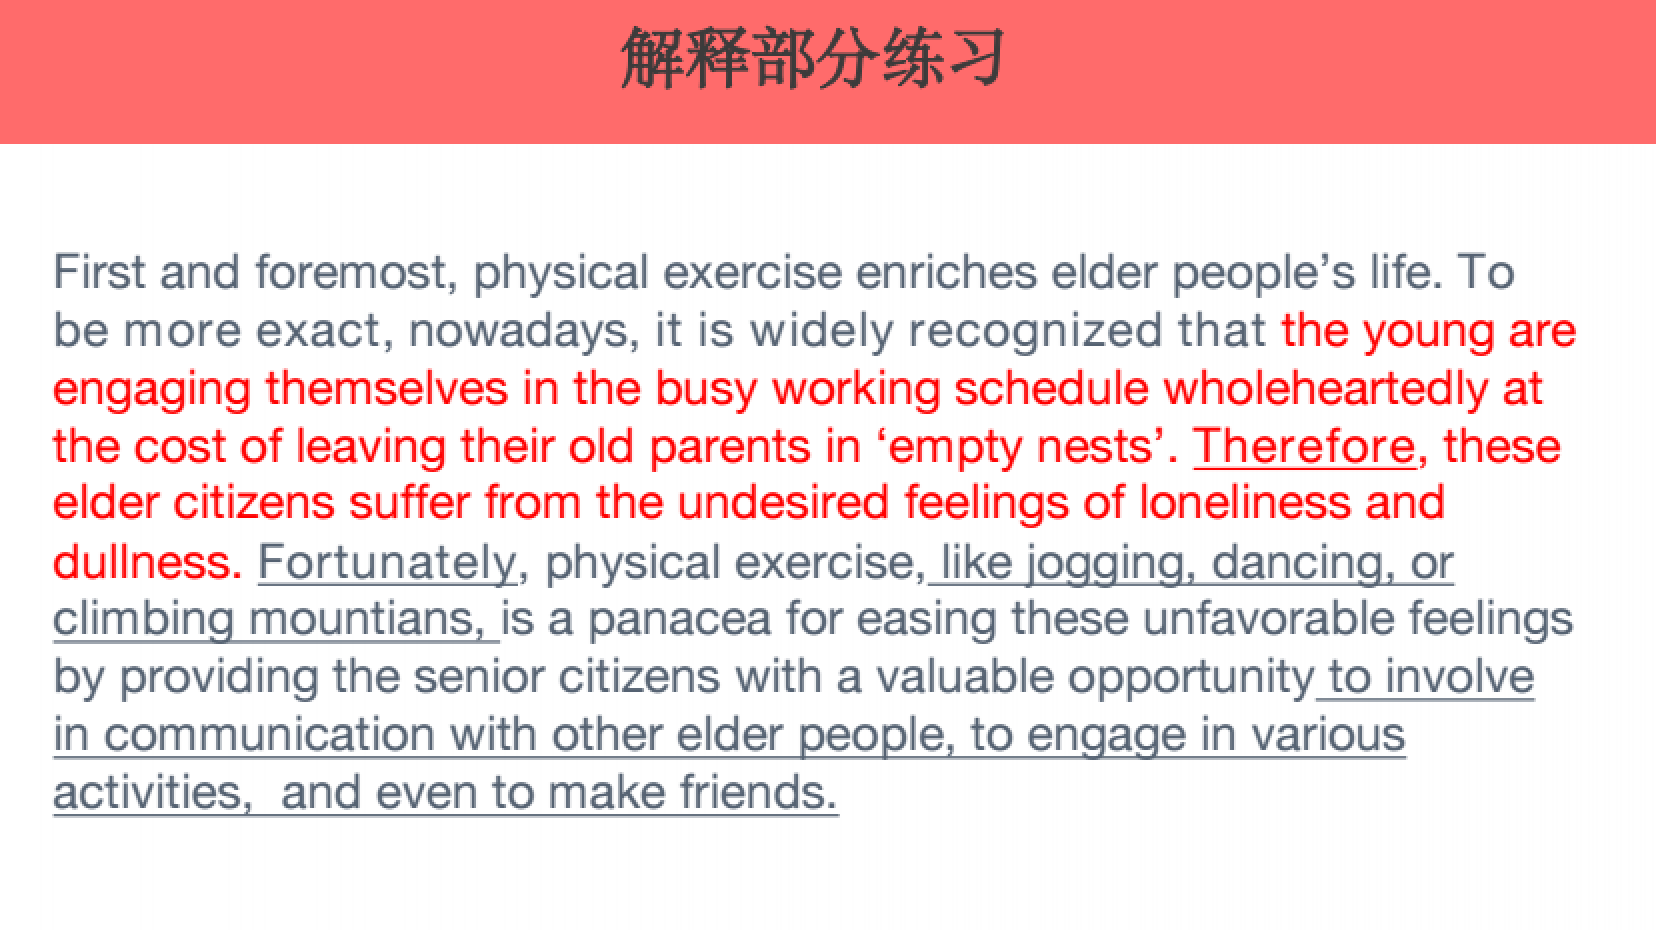
\includegraphics[width=4.00in,height=3.00in]{xiezuo12.png}
        \caption{例子}
              \end{figure}
                      \begin{figure}[!htp]
        \centering
        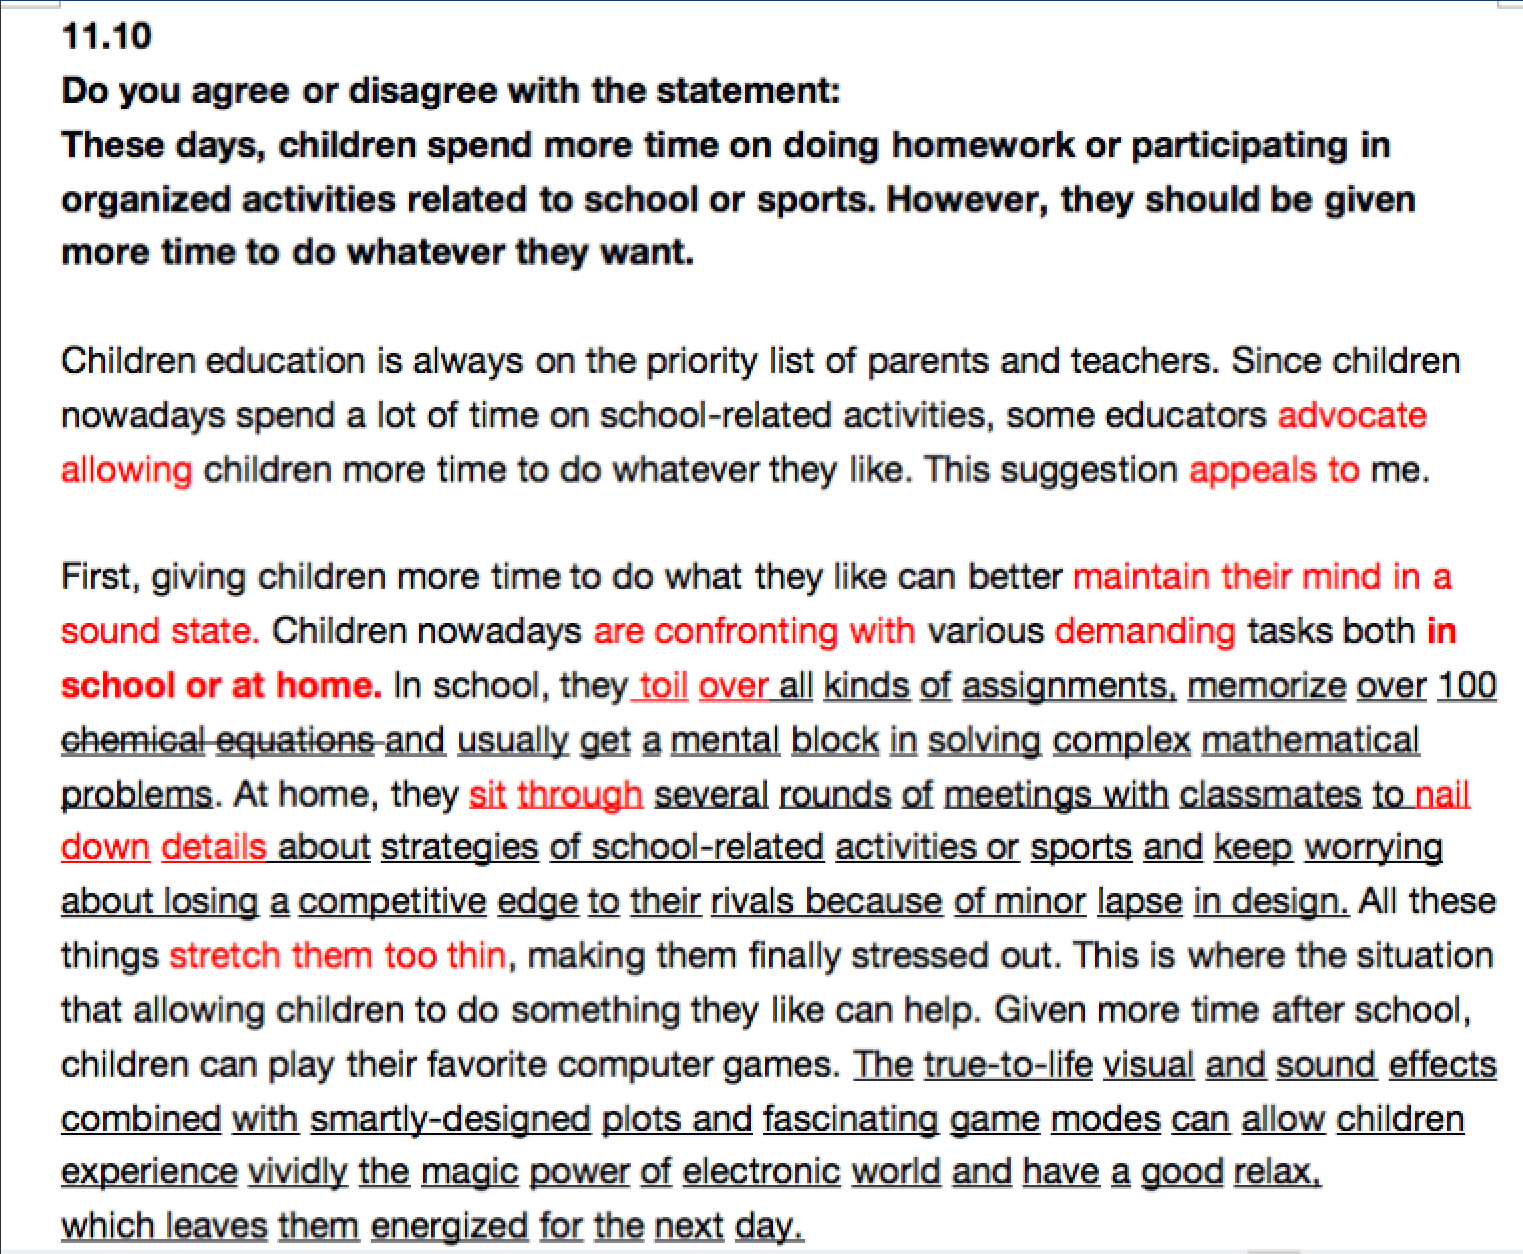
\includegraphics[width=4.00in,height=3.00in]{xiezuo13.png}
        \caption{例子}
              \end{figure}
      \item 引入以后,可以展开一下
      \item 通过写作真经,可以背诵每个类型一些话题引入的句子
      \item 遇到too much等极端词,分情况讨论
      \item 不要论证太故事化,不要第二人称,压缩题干(主题句)
      \item 主题句,分成AB..方面,后面细化A,B..
      \item 不仅要拆成两个方面,这两个方面还要再可以拆分,关键是细化,而不是重复解释,需要展开(介绍一下因果逻辑)但不要展开太长
      \item 例子\\
      解释部分:道理解释/普遍性解释\\
      举例部分:一个人一件事\\
      外国名人 、个人经历举例\\
      outline:起因(问题)、经过(观点)、结果(好处)\\
      主次分明  0.5-2 2-4 0.5-2 一共3-6句话,4句话就好\\
      细节: 具体化时间地点人物 数字 并列细节\\
      \item 词汇\\
        hone skill 锻炼技巧\\
        highly qualified teacher 很好的老师\\
        deprive sb. of sth.\\
        we may refer to 举例常用引语\\
        so but and 放在句中,不是前面\\
    \end{itemize}
    \item 解释\\
    \item 今昔对比\\
    1、两个大面对比\\
    2、细节不要简单的否定和被否定(表达上加直接not),要加上细节\\
    in the past, a great many of people made a living by farming or weaving, working for the whole day but just make ends meet. And there were still abundant people struggled at the verge of starvation at that time, not to mention to help others. nowadays,people's living standards are constantly improving, people's salaries are increasing,and they have surplus money to help those in need.Such as children who have no money to go to school and people who are sick and need to pay for medical expenses
    \item 结尾段=观点重申+分论点重写
  \item 综合写作
  \begin{itemize}
    \item 2
  \end{itemize}
\end{enumerate}
\section{口语}
\subsection{改革以后题型的变化}
删除第一题和第五题,花在背诵万能理由上的时间似乎可以减少,而练习听力复述的时间似乎可以增加。
\subsection{题型}
\subsubsection{第一题}
\subparagraph{Tips}
  \begin{itemize}
    \item 列出自己熟悉的话题,并根据它们进行练习。不妨从描绘一个熟悉的地方或者一段个人经历开始。注意在对话题进行详细描述的同时,一定要给出理由,例如为什么那件事很重要,为什么喜爱那件事情,以及那件事情是怎么影响你的。考生的回答中必须包括细节描述或事例。
    \item 描述的过程中不要列举过多内容,否则会减少有限的作答时间。在准备的15s过程中考生可以简单写下想说的内容,但切莫试图写出一篇完整的答案:一方面时间不允许;另一方面,评分人想考察的是考生对于这个问题能“说”的怎么样,而不是对于所写的东西朗读得怎么样。正式答题不要过分依赖写下的内容。
    \item 不要在考前死记硬背范文,尤其是在网上找到的,会降低分数。评分人可以轻松判断出是背诵的范文还是自然的回答,两者的节奏,语调甚至作答的内容有很大区别。
  \end{itemize}
  \textbf{例子讲述一个你最钦佩的老师并说说为什么钦佩他}\par
  先简略介绍一下所谈论的那个教师,要给出足够的信息。比如:他是教什么课程的;他教授你课程时,你多大年龄等等。然后陈述自己钦佩老师的原因。如果原因是做的具体事情——考生必须描述一下具体事迹,并且提供细节说明为什么她的行为可敬。也可能是这位教师表现出了很独特的个人品质,或者拥有很与众不同的性格特点——那么考生就要对此展开描述,例如你注意到她的这种行为的场合、其个人品质给你带来的影响等等。
\subsubsection{第二题}
\subparagraph{题目描述}
屏幕上出现两种可能的行为,需要考生谈论更喜欢哪一种行为或者情景,并谈谈作出这种选择的原因,即用理由、解释、细节或事例来支持自己的回答。一定要对问题的各个方面进行全面的回答,自己的观点应该十分清楚,并且要给出作出某个选择的理由。
\subparagraph{Tips}
\begin{itemize}
  \item 一个非常好的训练方法是自己陈述一个观点或一个偏好,然后给出清晰的理由和细节进行支持。在15s准备的时间不要试图写下所有的内容,只需要记下几个能够在作答过程中给予提醒和线索的单词胡总和短语即可。
  \item 学习常用的表达观点的单词和短语,如:In my opinion, I believe...
  \item 试着练习提出建议,并解释为什么。
\end{itemize}
\subsubsection{第三题}
\subparagraph{题目描述}考生会在电脑屏幕中读到一篇与校园生活有关的短文。考生会听到两个人谈论该话题,并且就短文中提到的话题发表自己的观点。接着考生要依据所读到的和所听到的内容回答一个问题。其中,阅读材料除了对提案的描述以外,阅读材料中还会列举两条要么支持要么反对该提案的理由。阅读材料的对话中,会听到两个学生谈论刚才读到的文章中的话题,其中之一会给出鲜明的观点——要么赞成,要么反对——并且还会给出理由支持自己的观点。问题有可能是根据听力和阅读材料中的信息说明这名学生的观点是什么,以及她/他给出了什么理由来支持自己的观点。\par
阅读材料提供上下文以便考生理解听力材料中对话者所谈论的话题,对话者只会间接的涉及阅读材料中的内容。因此阅读的过程中,考生必须对以下事情加以注意:提案的描述(即提出了什么,计划了什么,或改变了什么),以及支持或是反对该提案的理由。这将有助于考生在听对话时理解两个说话者到底在讨论什么。\par
在有些情况下,说话者会反对阅读材料中的某个立场,并且提供信息对材料中支持该立场的理由进行质疑。其他一些情况下,说话者会赞成阅读材料中的立场,并提供理由进行支持。因此,在听对话的过程中,考生必须明确说话者对于提案的观点,并且弄清楚说话者说的话和阅读材料中所获取的信息的关系。\par
考生不需要说明自己的观点,而是要陈述一个说话者的观点,并且总结说话者持该观点的理由。
\subparagraph{Tips}
\begin{itemize}
  \item 可以在托福考试的综合口语任务中就听力和阅读材料作笔记
  \item 尽量通过说话人的语调、重读和选词听出说话人的态度。这有助于理解他/她的观点并有助于考生规划自己的回答。
  \item 回答尽可能完整,能够使没看过这则通知或者没有看过这则对话的人在听了你的表达以后,也能够了解新的政策、女士的观点及她的理由。在阅读文章和对话中有很多信息,考生无需在回答中一一总结所有信息。
\end{itemize}
\subsubsection{第四题}
\subparagraph{题目描述}先阅读一篇学术类短文,然后听一个教授有关此话题的讲座的节选。之后=根据听力和阅读材料答题。时间时60s。考生回答这道题的手,需要依据短文和讲座中的信息并对其中的关键信息进行整合和表达。例如:有些题目中的短文对于一个总的规则或过程下了定义,讲座中谈到与此相关的一个具体例子或反例。这样的题目会要求考生用讲座中的具体例子解释短文中的规则或处理过程。另一种情况是短文描述了一个问题,而听力描述了针对该问题的一些或许成功或许失败,甚至会带来意想不到结果的解决方案。题目要求考生解释问题的解决方案并说明其结果。
\subparagraph{Tip}
\begin{itemize}
  \item 阅读一篇短文,把文中的主要观点列成提纲。使用提纲对短文进行口头总结。然后在提纲中加入细节,然后再进行口头总结
  \item 总结阅读次啊了和讲座中的所有信息,但是考生需要提供足够的细节信息,以便即使没有看过短文或没听过兼顾走的人也能理解你的表达。
\end{itemize}
\subsubsection{第六题}
\subparagraph{题目描述}首先要听教授就某一个学术问题所作讲座的节选,然后考生需要就此节选的内容答题。答题时间60s。通常教授开始会解释一个概念、强调一个问题或者介绍一种现象,然后讨论它的几个重要方面或与其相关的观点。讲座中会有一些说明性的例子来解释或阐明主要的概念或问题。题目主要是要求考生使用讲座中的观点和例子来说明其中的主要概念和问题。
\subsection{评分标准}
\begin{itemize}
  \item 总体陈述印象\\
  考生是否能做到清晰表达。好的表达应该流畅清晰、发音准确、语速适中、语音语调自然。
  \item 语言运用\\
  考生是否能有效利用英文语法和词汇来表达自己的思维。评分人会考察考生能够熟练运用简单和复杂的语言结构和恰当的词汇。
  \item 话题发展\\
  考生是否能完成命题所要求的任务,表达是否连贯一致。好的表达应该能够在规定时间内完成,并且能够让评分人很容易听出各个观点之间的关系和思想之间的衔接。
\end{itemize}
\subsection{如何训练口语}
\begin{itemize}
  \item complete?
  \item clear?
  \item grammatical error?
  \item use words correctly?
  \item organize idea clearly and appropriately?
  \item use time effectively?
  \item too fast? too slow? pause too often?
  \item 可以制作“口语日志”,用来存放自己的回答
\end{itemize}
\subsection{对于Rubric的解读}
\begin{enumerate}[A]
  \item Accuracy
  \begin{itemize}
    \item 同类型的错误不能过多
    \item 不影响理解
    \item 句子结构
    \item 语言是够地道
    \item 符合听力阅读
  \end{itemize}
  \item Diversity
  \begin{itemize}
    \item 高频词替换
    \item 句式替换
    \item 被动语态、形式主语、非谓语、there be
    \item 语气要有起伏
    \item 流畅度
    \item t发d音,th咬舌
  \end{itemize}
  \item Topic
  \begin{itemize}
    \item Details 自圆其说
    \item 综合口语的要点平均分布
    \item 综合超时会漏信息,独立没问题
  \end{itemize}
\end{enumerate}
\subsection{口语答题技巧}
\subsubsection{简写笔记}
  \begin{figure}[ht]
    \centering
    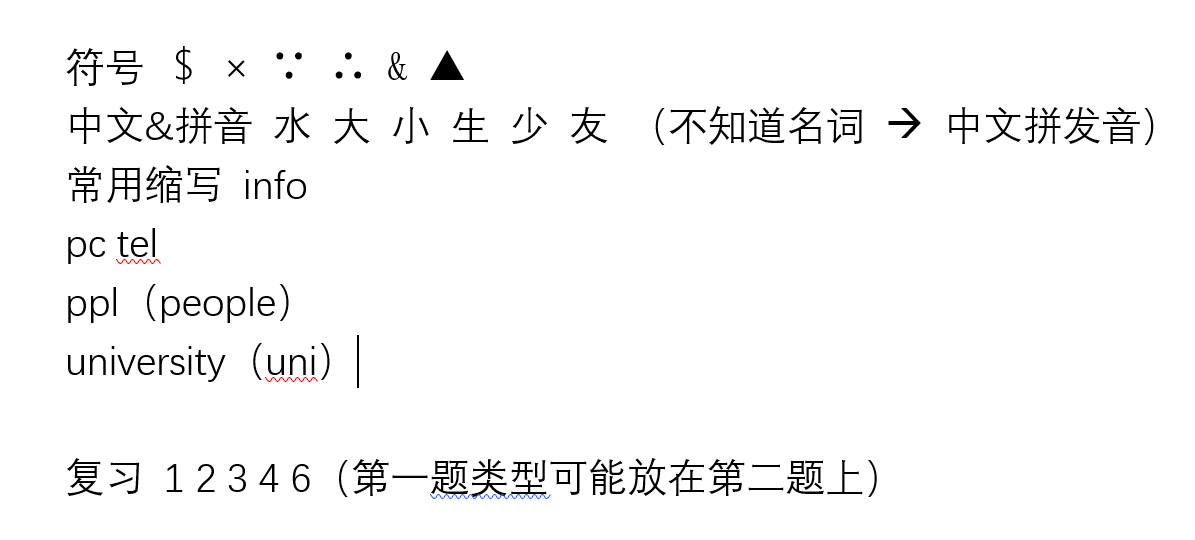
\includegraphics[scale=0.6]{kouyu1.png}
    \caption{常用符号}
    \end{figure}
\subsubsection{要求}
\begin{itemize}
  \item 练习以后,一定要改
  \item 计时
  \item 练习到ok才行
\end{itemize}
\subsubsection{Task 1}
\begin{enumerate}[A]
  \item Task 1\\
  1、要点不超过两个\\
  2、逻辑链、关键词\\
  3、先不要在意15s,先去写,慢慢减少\\
  4、最好撑满45s,实在不行that's why\\
  5、ABC 1+2+4句子 2+2一句 (1+2)*2\\
  \item 题型\\
    三选一、描述、建议、优缺点\\
  \item 答题框架\\
  \begin{itemize}
    \item 2+2\\
    1、三选一,所选项的一个优点,未选两项的缺点\\
    2、topic sentence 开篇点题\\
    3、Point 1+eg/explain\\
    4、linked words 逻辑\\
    5、Point 2++eg/explain\\
    6、构思的时候注意逻辑链\\
    \item ABC(分会高一点)\\
    1、A topic sentence\\
    2、because(非常必要)\\
    3、cite an example(experience/scenario)\\
    \item linked words\\
    that is/ in other words/ in case/ by doing so/ like/ such as
  \end{itemize}
\end{enumerate}
\subsubsection{Task 2}
\begin{enumerate}[A]
  \item 题型\\
  1、agree/ disagree\\
  绝对词,一定要回答否定\\
  2、which one better and why? (双条件题要把两个条件都考虑上)\\
  \item 结构\\
  看图\\
  具体化--名字 Bill Jennifer 年龄 7岁 地点 basketball court soccer pitch/field 足球场 Wanda plaze万达广场 \\
  \item 同义替换\\
  prefer --> my preference goes to / there is no doubt that A is better / doing A is more attractive \\
  agree --> vote for / be for / support / good idea\\
  oppose --> vote against / oppose
  \item 捧一个*2 踩一个,捧一个\\
  \item 句式\\
  I think the former one /latter one is better,...is more preferable\\
  I'm not in favor of the statement\\
  on the other hand... 否定\\
  必修课 Compulsory course 选修课 optional course\\
  appellation 称呼 honorific 敬语 \\
  节约时间,如果有想法就直接agree/disagree,不用重复题目了\\
  15s想不到第二点,就尽量想一个长一点的事例\\
  提问是第二人称,考生应该用I回答,讲道理时用we\\
  \item 一些套路
  \begin{itemize}
    \item 总起句+展开+重要性\\
    first, there are many things to do in the city. \textbf{To be specific/to illustrate,}big cities have libraries, museums, parks, amusement parks, and many other fun places for children to visit. Since children get bored easily, big cities are great for them because there are lots of entertaining places.
  \end{itemize}
\end{enumerate}
\subsubsection{Task 3}
\begin{enumerate}
  \item 题目描述\\
  大多数情况是,一个改变,两个理由;也有可能理由、变化、理由;很少数reason改变改变。\\
  \item reasons\\
  1、可行性\\
  2、disadvantage\\
  3、目的/好处\\
  \item 阅读时间不超过20s,两个原因点到即止,陈述一个观点,两条理由\\
  It is announced/informed by the university that   It is pro[osed by a student/ a professor that\\
  Reason Because More than that\\
  \item 如何记笔记\\
  1、记实词(名词动词形容词)\\
  2、合理利用符号\\
  3、汉字\\
  4、abbr 记前3-5个字母,去掉元音发音留辅音\\
  \item 句型
  
  she mention 
\end{enumerate}
\subsection{一些建议}
fiona 喜马拉雅fm 往清晰 流畅上面走 讲求性价比的话,不要追求高分 建议记笔记
\subsection{一些积累}
\begin{enumerate}
\item Task2
\begin{itemize}
  \item 要否定一个观点,先肯定正面的优点,再指出缺点,举例喜欢但不会去学习
  \item 时间有多余,therefore总结 / for this two reasons i prefer ...
  \item 连接词firstly sencondly 或者 on the other hand 至少举一个例子
  \item 陈述注重逻辑
  \item 如果题干比较长,就直接用prefer,不要陈述条件,会浪费很多时间
  \item 陈述前几句话的时候注意题目上的特定名词
  \item 记笔记不要让自己反应不过来
  \item 词汇
  \begin{itemize}
    \item that being said 话虽这么说
    \item Art sentiment 艺术情操
    \item become mature 变得成熟
    \item shape one's character塑造性格
    \item in a way 在某种程度
  \end{itemize}
\end{itemize}
\item Task3
\begin{itemize}
  \item 最好记下面,不要记标题
  \item 阅读材料只需要概括,一个举动,两个要点(词汇)即可
  \item 时态:一般现在时和过去式
  \item reading 记录 来自谁 topic r1 r2
  \item introduction的时候可以先把每个题的答题模板先写完
  \item 回答时间:阅读部分和听力部分之比 1:2 or 1:3
  \item 人称:第三人称单数 the man agrees
  \item 数字、时间和人名尽量详细的说上,学校名要加上
  \item plus 连接两个理由
  \item 对话者反对材料,解释她反对的理由
  \item 对话者 性别/名字 需要记录
  \item 一般fifteen,不会是fifty,人口没那么多
  \begin{itemize}
    \item The university is going to ... (in order to 可不加)... the woman doesn't agree with the plan/change. She says ...(理由) On the other hand, she claims that ...
  \end{itemize}
  \item 对话者支持材料,解释她支持的理由
  \begin{itemize}
    \item The university is going to ... in order to ... the woman likes this idea because firstly... (原因+结果). Secondly...
    \item The university plans to ... so as to ... and ... the woman thinks this change will work. She says ... also ... besides ...
    \item Also, she says this change will benefit the whole university. Since her friend's university started a similar change ...
  \end{itemize}
  \item 词汇
  \begin{itemize}
    \item Make money out of commercials 从广告中挣钱
    \item renovate new facilities 更新设施
    \item put them into a favorable position to find job 帮助他们找到工作
    \item so there is no worry that + 句子
  \end{itemize}
  \item 举例
  \begin{itemize}
    \item she mentions that her roommates..\\ 
  \end{itemize}
\end{itemize}
\item Task4
\begin{itemize}
  \item 出现冒号,破折号,前面的词是标题中的词语可能会是定义
  \item is called / known as / referred to as / is used to discribed /is that / is used to discribed
  \item 阅读记标题,记概念
  \item 指向性名词 phenomenon tendency ... + 定义句子 + when 的限制性条件
  \item xxx is a phenomenon that ... in the experiment ...
  \item xxx means ... for example ...
  \item xxx is an xxx who xxx ... in the professor's example of a painter called xxx, he says that ...
  \item according to the reading, outsider artist works ...
  \item 准备时间给自己的笔记填充逻辑关系
  \item 听力遇到不认识的单词直接记发音
  \item 阅读记 behavior/phenomenon(概念),主体(animals/people),句子(定义句子,有时候不一定只有一句)
  \item xxx is the ability to ... in the professor's first example, he says that ... and the second example is that ...
  \item reading找 名词+修饰
  \item 例子一般是一般过去时,除了生物。可能有一个例子,也可能两个 8句话
  \item 词汇
  \begin{itemize}
    \item be corresponding with 与...一致
  \end{itemize}
\end{itemize}
\item Task6
\begin{itemize}
  \item The lecture is mainly about two types of goods that ... one is called ... bacause ... for example ... and the other is ... for instance
  \item The lecture is mainly about two factors that make interior design more effectively. One is ... for example, and the other factor is ...
  \item Lots of animals developed different types of camouflage to help them hide from their predators.(总起) One of the camouflage is that ... take xxx for example ... and the second camouflage is that ...
  \item 七成都是生物
  \item 有可能不提到动物名,要求听出来/动物名词难度不大
  \item 出现的两种专业名词,题目会给
  \item 生物,一般现在时即可
\end{itemize}
\item 评分标准
\begin{itemize}
  \item sufficient(话题展开充分)\\
  1、不让考官提出问题\\
  2、数字、人名\\
  3、you人称不能出现\\
  \end{itemize}
\item 表达句型\\
表语从句,宾语,it is ... that,doing sth enables me\\
the first example is about a student who ...\\
  the second example is professor himself when ..\\
\end{enumerate}
\end{document} 